\documentclass[12 pt]{article}
\hbadness=10


\usepackage{amsmath, amssymb, amsfonts, setspace, stmaryrd, amsthm, graphicx, tikz}

\usepackage[utf8]{inputenc}
\usepackage[english]{babel}
\usetikzlibrary{positioning}% To get more advances positioning options
\usetikzlibrary{arrows}% To get more arrow heads
\usepackage{hyperref} % Allows to make references and links clickable

\usepackage[margin=1.5in]{geometry}
\newtheorem{theorem}{Theorem}
%%align* environment
\newcommand{\eq}[1]{\begin{align*}#1\end{align*}}

%Math commands
\DeclareMathOperator{\R}{\mathbb{R}}
\DeclareMathOperator{\C}{\mathbb{C}}
\DeclareMathOperator{\Z}{\mathbb{Z}}
\DeclareMathOperator{\N}{\mathbb{N}}
\DeclareMathOperator{\Q}{\mathbb{Q}}

\renewcommand\abstractname{Introduction}

\newcounter{exercise}[section]
\newenvironment{exercise}{\refstepcounter{exercise}\par\bigskip \begin{quotation}{}{\leftmargin .25in\rightmargin .25in}
	\noindent \textbf{Exercise~\thesection.\theexercise }  \rmfamily}{\end{quotation}\par\bigskip}
	

\newenvironment{bonus}{\refstepcounter{exercise}\par\bigskip \begin{quotation}{}{\leftmargin .25in\rightmargin .25in}
	\noindent \textbf{*Bonus Exercise*~\thesection.\theexercise }  \rmfamily}{\end{quotation}\par\bigskip}
	 


\title{RSA Cryptography}
\author{Girls Talk Math}
\date{}

\begin{document}
\maketitle
\vskip 1in
\begin{center} \textbf{Introduction} \end{center}

\indent In this problem set, you will learn about modular arithmetic, primes and RSA cryptography. Modular arithmetic and primes are classic topics in the area of number theory, a field of mathematics that has been a rich source of research for several hundred years and still remains very active. One particular development that grew out of number theory was the development of RSA encryption, a particular application of topics of modular arithmetic and primes well suited to the modern era.\\
    
    One goal of this problem set is to develop the tools necessary to learn and apply RSA encryption. By learning the associated theory behind this application, you will also learn about some of the fundamental properties of integers.
    
    One last note about reading mathematical texts: it is very normal when reading math to read a passage or even a single sentence several times before understanding it properly. Also, never trust the author! Check every claim and calculation (time permitting). Take your time and never give up. Let's talk math!
	
\newpage

\tableofcontents

%%%%%%%%%%%%%%%%%%%%%%
%%% Use \section{}, \subsection{}, etc. for different parts of the problem set. Start a newpage for a new section
%%%%%%%%%%%%%%%%%%%%%%

%%%%%%%%%%%%%%%%%%%%%%%%%%%%%%%%%
%%%
%%% Embed exercises in section as appropriate 
%%% 
%%%%%%%%%%%%%%%%%%%%%%%%%%%%%%%%%%%

\newpage


\section{Modular Arithmetic}
\subsection{Introduction}
This section is foundational for everything to come (and is useful in many areas of mathematics and computer science).

Let's rephrase what you already know about division with remainder. For any integers $n,d$ there are unique integers $q,r$ such that $n=qd+r$ such that $0 \leq r<d$. By unique, we mean that this pair $q,r$, and only this pair satisfy the above properties. You may have called $n$ the dividend, $d$ the divisor, $q$ the quotient, and $r$ the remainder. For example, $5=1\cdot3+2$ and $29=2\cdot 13+3$. In the first case, 3 goes into 5 once, with a remainder of 2. In the second case, 13 goes into 29 twice, with a remainder of 3.

On many occasions we only care about the remainder after division. For instance, consider an analog clock (shown in figure \ref{fig:clock}). If it reads 5 o'clock, what time will it read in 134 hours? Well, since the clock displays 12 hours in a circular manner, the clock has the same display every 12 hours. We want to find how many times 12 goes into 5 + 134 and determine the remainder. The resulting remainder will be the time of day. We can solve this problem by simply dividing by 12: $5+134=11\cdot12+7$.  So the clock will read 7 o'clock. This is an example of modular arithmetic in action.
\\
\begin{figure}[h]
\begin{center}
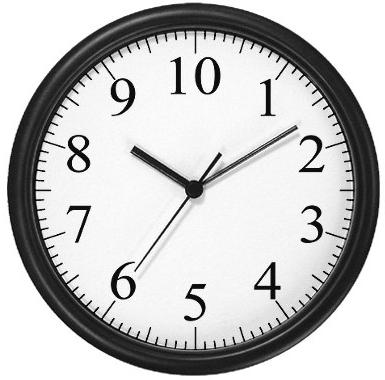
\includegraphics[width=0.4\textwidth]{GTM_Clip_Art_Clock}
\caption{12-hours Analog clock.}
\label{fig:clock}
\end{center}
\end{figure}
\\
Another example is the basic concept of odd and even. A number is even if its remainder when divided by 2 is 0 and is considered odd if this remainder is 1.

\subsection{Notation}
We will change notation later to emphasize a different aspect but this notation is standard in all of mathematics. Let $a,b$ be integers and $n$ be a nonzero integer. We write $a\equiv b\text{ mod }n$ (and we read ``$a$ is congruent to $b$ mod $n$'') if $a$ and $b$ have the same remainder when we divide by $n$. Rephrasing this in an alternative, yet equally correct manner, $a \equiv b\ (\text{mod } n)$ holds if there is no remainder after dividing $a - b$ by $n$.

\subsection{Finiteness}
Notice that when we divide an integer by $n$ the remainder is always an integer between 0 and $n-1$. Therefore every number is congruent modulo $n$ to a number between 0 and $n-1$ (the notation we use for modulo $n$ is $(\text{ mod } n$)). This finiteness is one reason modular arithmetic is so useful: to check a property for all integers modulo $n$ we only need to check it for the integers 0 to $n-1$.

\subsection{Arithmetic}
Let's look at some examples of how remainders behave upon addition and multiplication. Note that $29=2\cdot 13+3$ and $100=7 \cdot 13+9$ which means $29\equiv 3\ (\text{mod } 13)$ and $100\equiv 9\ (\text{mod } 13)$. Observe that
\[
100+29=129=9\cdot13+12,
\]
and that $12=3+9$. Thus in our notation $100+29\equiv 9+3\ (\text{mod } 13)$. That is to say, addition is preserved by taking remainders. The same is true for multiplication:
\[
100\cdot29=2900=223\cdot13+1.
\]
This means $100\cdot29\equiv 1\ (\text{mod } 13)$ and $9\cdot 3=27=2\cdot 13+1$ so we have that $9\cdot 3\equiv 1\ (\text{mod } 13)$. Therefore $100\cdot29\equiv 9\cdot3\  (\text{mod } 13)$ and so we see that multiplication is also preserved by taking remainders.

Since our usual operations on numbers are preserved by taking remainders and since there are only finitely many such remainders this motivates the following new structure which we call ``the integers$\mod$ $n$'' and we denote it $\Z_n$.

Fix a positive integer $n$. Consider the set of symbols $[0],[1],...,[n-1]$.  We define operations on these symbols via taking remainders:

\begin{center}
\begin{enumerate}
\item $[k]+[l]=[$\text{remainder of }$k+l$\text{ when divided by }$n]$
\item $[k]\cdot[l]=[$\text{remainder of }$k\cdot l$\text{ when divided by }$n]$
\end{enumerate}
\end{center}

While the notation is different from before, this is just expressing the same idea of congruence modulo $n$.

For example, if $n=13$ then we consider $[0],[1],[2],[3],[4],[5],[6],[7],[8],[9],$\linebreak$[10],[11],[12]$ with rules 1 and 2 above. Some sample calculations (check these!) are
\[
[10]\cdot[11]=[6]
\]
and $[12]+[12]=[11]$.

\begin{exercise}
Let $n = 12$ and compute the following:

\begin{enumerate}
\item $[5]+[7]$
\item $[6] + [11]$
\item $[15] + [27]$
\item $[8]\cdot [6]$
\item $[15]\cdot [10]$
\item $[27]\cdot [38]$
\end{enumerate}

Now, let $n = 13$ and compute the following:

\begin{enumerate}
\item $[5]+[7]$
\item $[6] + [11]$
\item $[15] + [27]$
\item $[8]\cdot [6]$
\item $[15]\cdot [10]$
\item $[27]\cdot [38]$
\end{enumerate}
\end{exercise}

Often times we will abuse notation and write a number larger than $n-1$ in brackets then reduce it modulo $n$. For example, in $\Z_5$ we may write 

\[[3]+[3]=[6]=[1]\] 
because  $6\equiv 1\ (\text{mod } 5)$. Also, we use the notation $k[l]$ to indicate the sum of $[l]$ with itself $k$ times. Note that $[-k]=-[k]$ because 
\[[-k]+[k]=[\text{remainder of k-k}\ (\text{mod } n)]=[0] \]

\textbf{Remark:}
If you wish you can think of the symbol $[k]$ as the set of all integers which are congruent to $k$ modulo $n$. Also, some people like to imagine $\Z_n$ as a ``number circle'' since $[n-1]+[1]=[0]$ and so adding $[1]$ to itself repeatedly cycles through all elements of $\Z_n$. Compare this to our discussion about clocks at the beginning.\\

\section{Primes}

The importance the role of primes serve, both in modular arithmetic and elsewhere in mathematics, cannot be overstated. In the following subsection, the exercises you complete may give you an idea of just one of the many nice properties that primes enjoy in the realm of modular arithmetic.  We explore further some properties of primes, with which it will be possible to use modular arithmetic in solving more complicated problems.


A \textbf{prime} number $p$ is a positive integer for which the only factors are 1 and $p$. By convention, 1 is not considered a prime.  By a factor of a given integer $n$, we mean an integer $m$ that integrally divides $n$, that is $n = ml$ for some integer $l$. 

\subsection{$\Z_p$ when $p$ is prime}
When we consider $\Z_p$ when $p$ is prime, $\Z_p$ has a property that makes it even closer to behaving like regular numbers. This is the following:
\begin{center}
For every element $[n]\not =[0]$ in $\Z_p$, there is another element $[m]$ such that $[n]\cdot [m]=[1]$. We call $[m]$ the \textbf{multiplicative inverse} of $[k]$.
\end{center}
For example, we have already seen that $[9]\cdot[3]=[1]$ in $\Z_{13}$. Typically, we denote the multiplicative inverse by using $-1$ as an exponent e.g. $[9]^{-1}=[3]$ in $\Z_{13}$. 

The notion of multiplicative inverse is present outside of the world of modular arithmetic. For example, it is satisfied by the rational, real and complex numbers. The idea, expressed in these contexts, is that for every element $a$ not equal to zero, there is another element $b$ such that the product $ab$ of these elements is equal to 1. For example, in the real numbers, the inverse of $9$ is $1/9$; the inverse of $1+i$ in the complex numbers is $\frac{1}{2}-\frac{1}{2}i$ where $i^2=-1$ (verify this!).

\begin{exercise}
Compute $[3]^{-1}$ in $\Z_5$ and $\Z_7$.
\end{exercise}

\begin{exercise}
In $\Z_4$, show that $[2]$ does not have an inverse. Note that 4 is not prime.
\end{exercise}


\subsection{Prime Factorization}

Continuing on with classifying positive integers, if a number $n$ is not prime, it is called a \textbf{composite} number and can be written as the product of two integers $2 \leq a \leq b < n$, $n = ab$.  We say an integer $c$ \textbf{divides} $d$, denoted by $c|d$, if there is an integer $l$ such that $d = lc$. In the case of composite $n$, we say that $a|n$ and $b|n$. Prime numbers have a special property when dividing a product of integers.  If $p$ divides the product of integers $a$ and $b$, written $p|ab$, then $p$ divides $a$ or $p$ divides $b$ (or $p$ divides both $a$ and $b$).  For example, $5|10\cdot 3$ and $5 \nmid 3$, but $5|10$. 

\begin{exercise} Prove the following statements. Let $a,b,c,d$ be integers with $a \neq 0$.\\

i) If $a|b$ and $a|c$, then $a|b + c$.\\
\indent ii) If $a|b$, then $a|db$.\\
\indent iii) For this, also assume $b \neq 0$. If $a|b$ and $b|c$, then $a|c$.
\end{exercise}


\begin{exercise}
Find an example of a composite number $a$ and non-zero integers $b$ and $c$ such that $a|bc$ but $a \nmid b$ and $a\nmid c$.
\end{exercise}

A consequence of this property of primes is the ability to factor integers into a unique product of powers of primes. 

A factorization of an integer $n$ into primes is a way of writing $n$ in the following form; $n = p_1^{a_1}\cdot p_2^{a_2}\cdots p_k^{a_k}$ where $p_1, \dots, p_k$ are distinct primes and $a_1, \dots, a_k$ are integers with $a_i \geq 0$ for $i = 1, \dots, k$. For example, $60 = 2^2 \cdot 3^1 \cdot 5^1$.
\\

\begin{theorem}[The Fundamental Theorem of Arithmetic]
If $n$ is an integer greater than 1, then $n$ can be written  as the product of primes.
\end{theorem}


The following is a proof of the above statement.  While useful to include, a complete understanding of it is not necessary for the subsequent material. 
\\

First observe that this holds for 2 as it is already a prime.  Assume we can factor the positive integers $k$ which are less than $n$ into a product of primes.  If $n$ is a prime, it is its own factorization.  If $n$ is a composite, then $n = ab$ where $2 \leq a \leq b < n$. Since we assumed that all integers $2 \leq k < n$ have prime factorizations, $a$ and $b$ have such factorizations.  Then, taking the product of these factorizations yields a factorization of $n$.

To show uniqueness, suppose there are two such factorizations $n = p_1^{a_1}\cdots p_k^{a_k}$ and $n = q_1^{b_1}\cdots q_l^{b_l}$.  Then $p_1^{a_1}\cdots p_k^{a_k} = q_1^{b_1}\cdots q_l^{b_l}$.  Since $p_1$ divides the left hand side, it divides the right hand side.  Since $p_1$ is a prime and the right hand side is a product, it must divide one of $q_1, \dots q_l$, say $q_j$. Since $q_j$ is a prime, it must in fact be $p_1$ and since $p_1^{a_1}$ divides the left hand side, dividing by $p_1$ $a_1$ times means $b_j \geq a_1$.  Continuing this process, we divide out by all the primes on the left hand side until it just equals 1.  The right hand side will be a product of primes raised to powers, all of which are necessarily zero. Hence, the $q_i$ are in fact the $p_l$ possibly reordered, but with the same corresponding exponents and thus the factorization is unique.  

\begin{exercise}
Factor the following integers into a product of powers of primes:

\begin{enumerate}
\item 15
\item 38
\item 97
\item 147
\item 184
\item 216
\end{enumerate}

Hint: When trying to find factors of some positive integer $n$, we need only check the integers $k$ between 1 and $\sqrt{n}$.  For instance, if $n = 59$, we only need to check only the integers $1,2,3,4,5,6,7$.  Since none of these divide $59$, we conclude $59$ is prime. Similarly, for $n = 77$, we see need to test integers between $1, \dots, 9$ for a factor.  Since $7$ is a factor, we see $77 = 7 \cdot 11$ and since $11$ is a prime, we are done. The reason for this is that if $n = ab$ and $a \leq \sqrt{n}$ then it must be the case that $b \geq \sqrt{n}$.  Thus, if no factors exist less than $\sqrt{n}$, then no factors exist greater than $\sqrt{n}$.

\end{exercise}

\subsection{Greatest Common Divisor}

With a unique factorization into primes for each integer, one may ask about when two integers share factors in common. This brings into view the idea of the greatest common divisor, $d = \gcd(a,b)$, of two integers.  This integer has the special property that $d|a,\ d|b,$ and if $r|a$ and $r|b$ for some integer $r$, then $r|d$.  

\begin{exercise}
Write out the prime factorizations for 12 and 18.  Calculate $\gcd(12,18)$ and write out its factorization.  Compare the three factorizations.  What do you notice about the exponents?
\end{exercise}

If we write $a = p_1^{a_1}\cdot p_2^{a_2} \cdots p_k^{a_k}$ and $b = p_1^{b_1} \cdot p_2^{b_2} \cdots p_k^{b_k}$ where the $p_i$ are distinct primes and $a_i,b_i \geq 0$, and let $m_i = \min(a_i,b_i)$ the minimum of the two exponents for the prime $p_i$, then $d = \gcd(a,b) = p_1^{m_1}\cdot p_2^{m_2} \cdots p_k^{m_k}$.  In the preceding exercise, the prime factorizations for 12 and 18 are $2^2\cdot 3$ and $2 \cdot 3^2$ respectively.  One can calculate that $6 = \gcd(12,18)$ with prime factorization $6 = 2 \cdot 3$.

We say two integers $a,b$ are \textbf{relatively prime} if $\gcd(a,b) = 1$.  Notice, $a$ and $b$ need not be prime themselves; for example if $a = 35$ and $b = 8$, then $\gcd(a,b) = 1$ but neither integer is prime.

\begin{exercise}
Calculate $\gcd(a,b)$ for the following pairs of integers $a,b$: i) $a=1, b= 15$, ii) $a = 8, b = 12$, iii) $a = 24, b = 25$, iv) $a = 0, b = 28$. 

Which of the previous pairs are relatively prime?
\end{exercise}

One may ask how many integers $1 \leq k \leq n$ are relatively prime to $n$.  The Euler $\varphi-$function counts this. Euler, pronounced "Oiler" was an influential mathematician in many areas, including number theory.
$\varphi$ is a Greek letter pronounced "fee". In technical terms, $$\varphi(n) = |\{k \in \mathbb{Z}^+| 1 \leq k \leq n,\ \gcd(k,n)=1\}|$$
The previous expression needs some unpacking.  If $A$ is a set, $|A|$ denotes how many elements are in the set; this can be finite or infinite. $\{\cdot\}$ is set notation. Hence, $\{ k \in \mathbb{Z}^+\}$ is the set of all positive integers $k$ (that is because $\mathbb{Z}$ is the symbol for the integers set). The vertical bar in the curly brackets is read as "such as". So the above expression is, "the set of positive integers $k$ such that $k$ is between 1 and $n$, and $k$ and $n$ are relatively prime." Remember that two numbers $k$ and $n$ with gcd($k,n$) = 1 are relatively prime.

\begin{exercise}
Compute $\varphi(1), \varphi(2), \varphi(3), \varphi(4), \varphi(5),\ldots, \varphi(25)$ and list these in a table.  

For example, $\varphi(6)$ is the number of integers $k$ between 1 and 6 that are relatively prime to 6.  The integers 2, 4, 6 are all divisible by 2 and the integers 3, 6 are divisible by 3.  Since 1 and 5 only share the factor 1 with 6, these are relatively prime.  Hence, $\varphi(6) = |\{1,5\}| = 2$.\\

{\tiny\begin{center}
\begin{tabular}{|c|c|c|c|c|c|c|c|c|c|c|c|c|c|c|c|c|c|c|c|c|c|c|c|c|c|c|}
\hline
     $n$& 1&2&3&4&5&6&7&8&9&10&11&12&13&14&15 \\
     \hline\\[-3ex]
     $\varphi(n)$& & & & & & 2& & & & & & & & &   \\
     \hline
\end{tabular}
\end{center}}

{\tiny\begin{center}
\begin{tabular}{|c|c|c|c|c|c|c|c|c|c|c|c|c|c|c|c|c|c|c|c|c|c|c|c|c|c|c|}
\hline
     $n$&16&17&18&19&20&21&22&23&24&25 \\
     \hline\\[-3ex]
     $\varphi(n)$ & & & & & & & & & &   \\
     \hline
\end{tabular}
\end{center}}


Do you see a pattern with $\varphi(p)$ for primes $p$? Why do you think this is the case? Come up with the value of $\varphi(p)$ if $p$ is a prime.
\end{exercise}

\begin{exercise}
\begin{itemize}
\item[i)] What are $\varphi(15)$, $\varphi(3)$ and $\varphi(5)$? Can you relate $\varphi(15)$ to $\varphi(3)$ and $\varphi(5)$?\\

\item[ii)] How about $\varphi(91)$ in relation to $\varphi(7)$ and $\varphi(13)$?\\

\item[iii)] Now consider $\varphi(24)$ in relation to $\varphi(4)$ and $\varphi(6)$?  How about $\varphi(24)$ in relation to $\varphi(3)$ and $\varphi(8)$?\\

\item[iv)] How are the pairs $3$ and $5$, $7$ and $13$ similar to the pair $3$ and $8$? And how are they not similar to the pair $4$ and $6$?
\end{itemize}
\end{exercise}

\begin{exercise}
Suppose that $p,q$ are distinct primes. Suppose $n$ is an integer such that $\gcd(n,pq) \neq 1$. What are the possible factors of $pq$? Since $\gcd(n,pq) \neq 1$, what are the possible values of the $\gcd(n, pq)$? What can you conclude about $n$?
\end{exercise}

\begin{exercise}
If $p,q$ are different primes, what do you think $\varphi(pq)$ is in terms of $\varphi(p)$ and $\varphi(q)$?  Look at the examples in your table.  When you have a guess, try counting the number of integers $1 \leq k \leq pq$ which are divisible by $p$. Then count the numbers divisible by $q$.  Finally, count the number of integers divisible by $pq$.  The goal here is to determine how many integers between 1 and $pq$ are divisible by $p$ or $q$ (or both). It might be helpful in doing this to keep in mind the previous exercise. Consider listing out the integers. If you have double counted, make sure to correct this error.  Subtract the number of such integers from $pq$, the total number of positive integers between 1 and $pq$, to determine the integers relatively prime to $pq$.  What is this number in terms of $\varphi(p)$ and $\varphi(q)$? This is the value of $\varphi(pq)$.
\end{exercise}

One of the interesting properties of the Euler $\varphi-$function is the following statement. 

\begin{theorem}[Euler $\varphi-$Theorem] Let $a,n$ be positive integers that are relatively prime. Then, $a^{\varphi(n)} \equiv 1 (\text{mod}\ n)$
\end{theorem}

This theorem is quite useful. In particular, when computing large powers of integers using modular arithmetic, we may simplify our calculations by using this identity if $\gcd(a,n) = 1$.

\begin{exercise}
Verify Euler's $\varphi-$Theorem for $n = 4$ and $a = 3$.  How about $n = 25$ and $a = 17$?  Try out a few more examples to see that this works.  What about the case of $n = 12$ and $a = 6$?
\end{exercise}

\subsection{Chinese Remainder Theorem}

\begin{theorem}[Chinese Remainder Theorem]
Suppose $n_1, n_2, \dots, n_k$ are relatively prime positive integers greater than 1.  Then $$\varphi(n_1n_2\cdots n_k) = \varphi(n_1)\varphi(n_2)\cdots \varphi(n_k)$$
\end{theorem}

We previously calculated that $\varphi(24) = 8$. Writing $24 = 3 \cdot 8$, and noting that $\gcd(3,8) = 1$, it is clear that $8 = 2 \cdot 4 = \varphi(3)\cdot \varphi(8)$. However, we also observed that $\varphi(6) = 2$ and $\varphi(4) = 2$, but $8 \neq 2 \cdot 2$. The equation in the theorem does not necessarily hold when the factors are not relatively prime.\\

We now explore some results which follow from this.

\begin{exercise}
If $n = p_1p_2\dots p_k$ where the $p_i$ are distinct primes, what is $\varphi(n)$? Verify this by calculating $\varphi(30)$. Recall that for $p$ prime, $\varphi(p) = p-1$.
\end{exercise}

Now, we consider a more generic integer, with higher multiplicities of primes. Before we do so, we define what it means for two integers to be pairwise prime.

Two integers are pairwise prime if they share no factors, i.e. $a$ and $b$ are pairwise prime if and only if $\text{gcd}(a,b) = 1$.  If $n$ is a positive integer, we say it is a product of pairwise relatively prime positive integers if $n = a_1\cdot a_2 \cdots a_k$ such that for $i \neq j$, $\text{gcd}(a_i,a_j) = 1$.

\begin{exercise}
The integers 20 and 36 can each be written as a product of pairwise relatively prime positive integers. Verify that $\varphi(20)$ and $\varphi(36)$ are the values predicted by the formula in the Chinese Remainder Theorem.
\end{exercise}

Now, we use the Euler $\varphi-$Theorem to verify a less obvious fact.  

\begin{exercise}
Let $n,p$ be relatively prime integers $n,p$ where $p$ is prime. Show that $p| n^{p-1} - 1$.  Recall, for integers $a$ and $b$, $a|b$ is equivalent to the existence of some integer $c$ such that $b = ac$. You will want to apply the Euler $\varphi-$ Theorem to the expression $n^{p-1} - 1$ modulo $p$.
\end{exercise}

Now, we consider a slightly harder application which builds off of the previous exercise.

\begin{exercise}
If $q$ and $n$ are relatively prime integers and $k$ is any integer greater than or equal to zero and $q$ is prime, use the Euler $\varphi$ theorem to prove that $q|n^{q+k} - n^{k+1}$. Recall that $x^px^q = x^{p+q}$ and consider factoring out a power of $n$ from $n^{q+k} - n^{k+1}$ to put it into a form similar to that found in the previous exercise.
\end{exercise}

We now consider some more applications in the following two exercises.  The intended purpose of these exercises is to familiarize yourself with the computation techniques available in modular arithmetic when there is sufficient relative primality between the integers in question.

\begin{exercise}
If $p$ and $n$ are relatively prime and $q$ and $n$ are relatively prime with $p$ and $q$ prime, use the Euler $\varphi$-Theorem to prove that $pq|(n^p - n)(n^{q+2} - n^3)$. Show that each prime divides something specific and then deduce the conclusion about their product.
\end{exercise}

\begin{exercise}
If $p$ and $n$ are relatively prime and $q$ and $n$ are relatively prime with $p$ and $q$ prime, use the Euler $\varphi$-Theorem to prove that $pq|n^{pq} - n^p - n^q + n$. Try factoring the expression $n^{pq} - n^p - n^q + n$ in a way that you have seen in the previous exercises.
\end{exercise}

Now, we use some clever divisibility tricks. The following exercises are trickier than the preceding ones.  They are not necessary for the material that follows, but are nevertheless a good opportunity to apply the theory you have learned up to now and should help develop a deeper understanding of the material overall.

\begin{exercise}
Prove that $7|10q + r$ if and only if $7|q - 2r$ where $q,r \in \mathbb{Z}$.  Recall that if $a|b$ and $a|c$ then $a|b+c$ and $a|b-c$ (and $a|c-b$ similarly).
\end{exercise}



\begin{exercise} Suppose a given integer $a$ has decimal expression $a = d_kd_{k-1}\dots d_0$, and define $a' = d_kd_{k-1}\dots d_1 - 2d_0$. Set $a'' = (a')'$, $a''' = (a'')'$ and so on. Show that $7|a$ if and only if some integer $a', a'', a''', \dots$ is divisible by 7 (in fact, this will hold for every integer in the collection $a', a'', a''', \dots$).  For example, if $a = 65464$, then $a' = 6546 - 8 = 6538$, $a'' = 653 - 16 = 637$, and $a''' = 63 - 14 = 49$; we conclude that $65464$ is divisible by 7. since $7|49$.
\end{exercise}

\begin{exercise}
Show that $1000 \equiv -1 (\text{mod } 7)$
\end{exercise}



\begin{exercise}
Suppose that we are given an integer written in the form $a = r_0 + 1000r_1 + (1000)^2r_2 + \cdots + (1000)^kr_k$ for integers $r_0, r_1, \dots , r_k$, i.e., $1,002,005,007 = 7 + 1000^1\cdot 5 + 1000^2\cdot 2 + 1000^3\cdot 1$. Show that $7|a$ if and only if $7|r_0 - r_1 + r_2 - \cdots + (-1)^kr_k$.  Recall that $a \equiv c\ (\text{mod } z)$ and $b \equiv d\ (\text{mod } z)$ then $a + b \equiv c + d\ (\text{mod } z)$ and $ab \equiv cd\ (\text{mod } z)$.
\end{exercise}


\newpage
\section{RSA Cryptography}
You should use Wolfram Alpha or a similar program to do the modular arithmetic. Wolfram Alpha is a website (wolframalpha.com) which can perform large calculations for you; if you wish to calculate $a$ (mod $N)$ just type ``$a$ mod$ (N)"$.

We saw in an earlier page that if the integers $a$ and $N$ are relatively prime, then $A^{(\varphi(N))} \equiv 1$ (mod $N)$.  Let's make a calculation about $a^{st}$ if $st\equiv 1$ (mod $\varphi(N))$, for a pair of integers $s$ and $t$.

\begin{exercise}  Given that $st \equiv 1$ (mod $\varphi(N))$, write a useful expression for $st$.

Now rewrite $a^{st}$ using your expression.  Demonstrate that $a^{st} \equiv a$ (mod $N)$.
\end{exercise}

We will use this fact in RSA encryption. Here's a full example of the RSA Algorithm:\\
Alice and Bob are trying to communicate secretly. They agree that they will use the cipher (making letters into numbers) via the following rule: $(1=a, 2=b, \dots 26=z)$. Alice picks two primes, say, 17 and 19. She multiplies these to get 323, which we'll call $N$. She then finds $\varphi(N)$, which we know (since we know $N=17\times 19$) is just $(17-1)(19-1) = 288$. Then she needs two numbers, $s$ and $t$, both of which are relatively prime to $\varphi(N)$ such that $s t \equiv 1$ mod $\varphi$(N). She then figures out that if $s=11$ and $t=131$, then $11\times 131 \equiv 1$ (mod 288).  These two numbers are not special; she just has to find two such numbers where the product is $1$ (mod 288) and such that both numbers are relatively prime to 288. 
\medskip

Then Alice sends $(s, N) = (11, 323)$ publicly to Bob. Eve is listening in, so she also has the information (11,323). Bob then wants to transmit the letter $U$ to Alice. In our cipher, this corresponds to the number 21. So Bob computes $21^s=21^{11} = 350277500542221$, and then (using a computer) calculates 350277500542221 (mod $323)$ and finds it to be 319. Bob then sends 319 to Alice. Eve is still listening so knows this as well. To decode, Alice takes 319 and raises it to the number $t=131$ to get $319^{131}$ which is a \textit{really} large number, but mod 323, it is 21, which corresponds to the letter U! Eve knows some information, but not the important stuff, so it would take her awhile to decode the message.

\begin{exercise}
Describe what additional information Eve should obtain if she wants to decode this message efficiently.
\end{exercise}
% There are two pieces of information necessary; $t$ and $\varphi(N)$. Calculating $\varphi(N)$ essentially means factoring the number 323 in this case. Factorization gets very difficult as the numbers become large, so this is a difficult step. Finding $t$ now means finding a number relatively prime to $\varphi(N)$ such that $t \cdot s=1$ modulo $\varphi(N)$. This is not as difficult as the step above. 
\medskip

Note that in the above example, Alice only receives the ``information'' of $a^s\ (\text{mod } N)$; however this is also all that she needs. Exercise 3.1 demonstrates that she will get the correct message simply by raising whichever number she gets to its $t$ power, and then reducing mod 323.

\medskip

Another important thing to see here is that Exercise 3.1 is vital to the success of this cryptography. With all of our assumptions in place on the numbers $s$ and $t$ relative to $\varphi(N)$, it is a fact that $a$ and $a^{st}$ are equivalent modulo $\varphi(N)$. Thus, since $a^{st}=(a^{s})^t$, as long as one knows $a^s$ modulo $\varphi(N)$ and $t$, one knows $a$ modulo $\varphi(N)$: simply take $a^s$ modulo $\varphi(N)$, raise it to the $t$ to get $a^{st}$, and reduce again (mod $\varphi(N))$. This will spit out $a$ again, no matter what! 


\begin{exercise}
  Let (s=7, t=7, N=35, $\varphi($N$)$=24).  Compute $2^7\ (\text{mod } 35)$, $4^7\ (\text{mod } 35)$ and $10^7\ (\text{mod } 35)$.  Then exponentiate all of these resulting numbers by $t=7$ again, and reduce modulo 35 again.  What do you get?  
\end{exercise}


Try your hand at the following encodings:

\begin{exercise} You know (s=7, t=7, N = 35 (=5$\times$7), $\varphi($N$)$=24). Decipher the following message: (28, 9, 32, 33, 19)  

Let's just examine the first letter.  A 28 as the first letter means Bob took some letter (number) a, and then examined $a^s=a^7 \equiv 28$ mod $(35)$.  Now recall by Exercise 3.1 just above that $(a^{s})^t \equiv a^{st} \equiv a\ (\text{mod } N)$.  Thus we examine $28^7\ (\text{mod } 35)$, getting 7.  Since $7$ corresponds to $g$, the first letter is $g$.  In this example, both $s=7$ and $t=7$; if we wanted to make a harder code we would pick much bigger primes (and they'd probably be different primes).
%Girls - take each number to the 7th power, then mod 35
\end{exercise}

\begin{exercise}  You know (s=7, t=7, N = 35 (=5$\times$7), $\varphi($N$)$=24). Decipher the following message: (20, 1, 33, 11)
%talk - take each number to the 7th power, then mod 35
\end{exercise}

\begin{exercise} You know (s=7, t=7, N = 35 (=5$\times$7), $\varphi($N$)$=24). Decipher the following message: (27, 1, 20, 22)
%math - take each number to the 7th power, then mod 35
\end{exercise}

\begin{exercise}  You know (s=7, t=679, N = 851 (=23$\times$37), $\varphi($N$)$=792). Decipher the following message: (828, 684, 453, 485, 701, 32, 684)
%welcome - take each number to the 679th power, then mod 851
\end{exercise}

In terms of calculation, these exercises have not been so bad.  But let's imagine that we are an outsider trying to crack the code. 

\begin{exercise}
If you saw Alice send the information $(s=7, N=35)$ and you saw Bob send back the number $28$, what information do you need to decode 28?
\end{exercise}

\begin{exercise}
 You know (t=23, N = 57, $\varphi($N$)$=36). Decipher the following message: (32, 3, 0, 3, 32, 44, 0, 26, 32, 3, 35, 19, 0, 35, 50, 1, 20, 0, 20, 50, 24, 19, 0, 19, 1, 55, 19)
%No one knows what this says - take each number to the 57th power, then mod 57
\end{exercise}

\begin{exercise}  You are now trying to encode a message. You are given $(s=31 , N=120 )$, how would you encode the message, ``Penguin''?
%{P, e, n, g, u, i, n} = {16, 5, 14, 7, 21, 14} Raise each number to the 31st and mod by 120 ---> {16, 5, 104, 103, 21, 104}
\end{exercise}

\begin{exercise} If you were Eve and listening in, if you saw that $N = 77$, what would the two prime numbers $p$ and $q$ have to be to give $N = 77$? What is $\varphi(N)$?
%N = 7x11 so Phi(N) = 6x10 = 60
\end{exercise}

\begin{exercise}  If you were Eve and listening in, if you saw that $N = 1591$, can you calculate $\varphi(N)$? 
%N = 37x43, so Phi(N) = 36x42 = 1512
\end{exercise}

\begin{exercise} If you were Eve listening in and you saw Alice send Bob $(s=13, N=77)$, and then you see Bob send Alice the code (61, 1, 49, 53, 23, 58, 38, 50), can you crack it?
%Sandwich
\end{exercise}

\begin{exercise}  Using the cipher $a=1, b=2, c=3 ...$, work with a partner to encode messages. First, one person use $N = 5 \times 7$, then find $\varphi(N)$, and appropriate $s$ and $t$. Give the other person $(s, N)$ and have them encode a message and send it to you. Then decode it. Next, switch roles. Now use $N = 7\times13$ and do the same thing.
\end{exercise}

\begin{exercise}  Can you find a number $t$ such that $4\times t \equiv 1$ mod(8)? What about such that $5\times t \equiv 1$ mod(8)? Can you find a number $N$ such that $\varphi(N) = 8$? 
\end{exercise}

\begin{exercise}
 Work with your team to come up with an $s$, $t$, $N$ and $\varphi(N)$ and your own cipher to encode a message with at least 25 letters in it (this can include spaces). Give the other team the information they would have if they were Eve \textemdash that is $s$, $N$ and the encoded message $m$. The first team to crack the other team's code wins!

Additional rules: 
1) Your cipher doesn't have to just mix up the numbers 0-26 or 1-27. For example, one could use 3-29. They don't even have to be sequential. However, you must have $\varphi(N)$ greater than the largest number in your cipher. 
2) Use primes greater than 13 and lower than 50 to get your $N$.
\end{exercise}






\end{document}
